\section{Results}
Use three datasets for which we have some ground truth. They are all small

Comparison: Pr* (Optimal single pipeline), RPr (All samples of EPS), RPr-50 (50\% of EPS samples), Pr- (worst pipeline), and baseline* (Jiannan's Crowder Clustering algorithm but using the best sequence of actions).

\subsection{Does Randomization Make Pipelining More Robust?}
Compare to best single pipeline, worst single pipeline, and current state of the art.
We should find that a randomized execution is much better than the worst and hopefully comparable to the best.
In some cases, it may be better than the best, but it should never be worse than the worst.

Dataset: MS Academic 
Operations: Filter and Deduplicate

Dataset: Yelp 
Operations: String Clean, City Format, Deduplicate

Dataset: Product 
Operations: identify sku if exists, string clean, Deduplicate

\begin{figure}[ht]
\centering
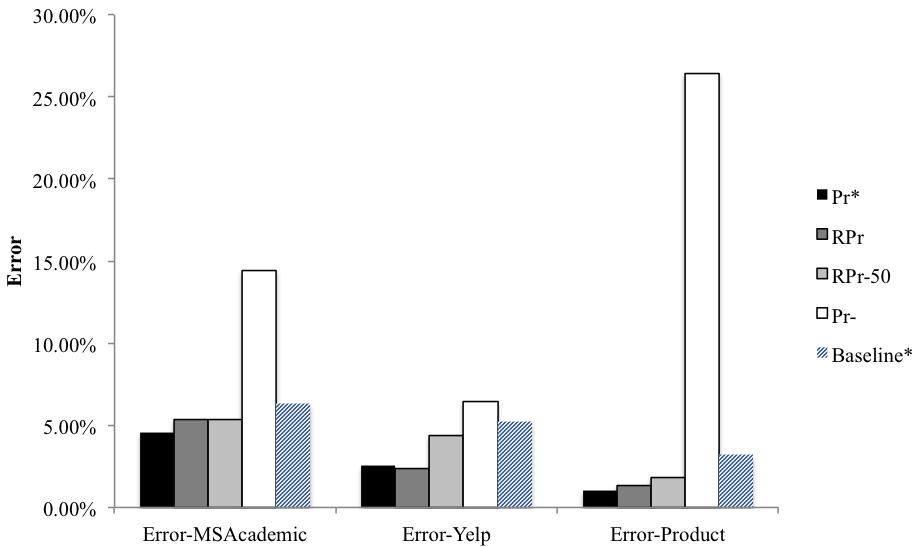
\includegraphics[scale=0.4]{fig1.png}
\caption{}
\label{exp:ms-academic-ranking}
\end{figure}

\subsection{How does this vary with random error in the operators?}
Should show that the more unreliable the data cleaning is the more that our approach benefits.

Introduce varying amount of random error (hashed so consistent between runs) into the ``city formatting" fix for the yelp dataset:

\begin{figure}[ht]
\centering
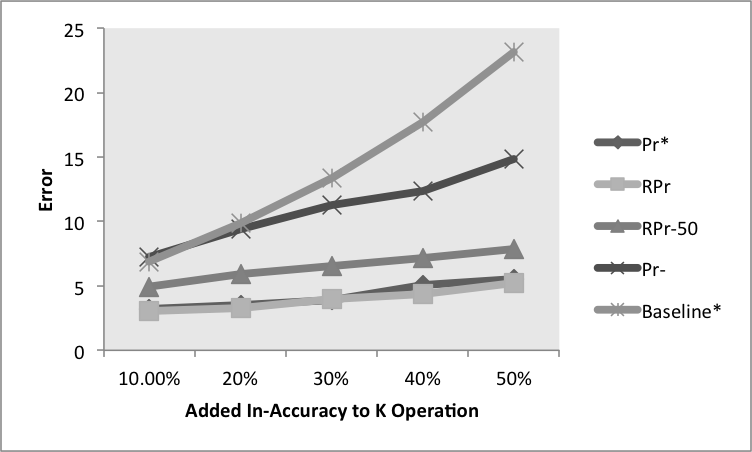
\includegraphics[scale=0.5]{fig2.png}
\caption{}
\label{exp:ms-academic-ranking}
\end{figure}

Introduce varying amount of random error (hashed so consistent between runs) into an extra dedup operation.

\begin{figure}[ht]
\centering
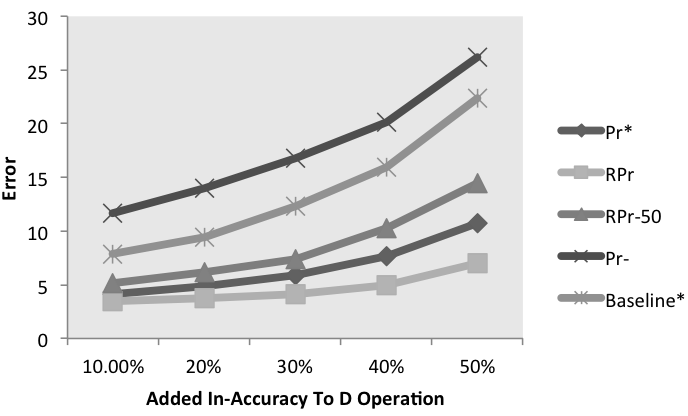
\includegraphics[scale=0.5]{fig3.png}
\caption{}
\label{exp:ms-academic-ranking}
\end{figure}

\subsection{Runtime-Accuracy Tradeoff}
Execute more samples and show how the accuracy improves.

\begin{figure}[ht]
\centering
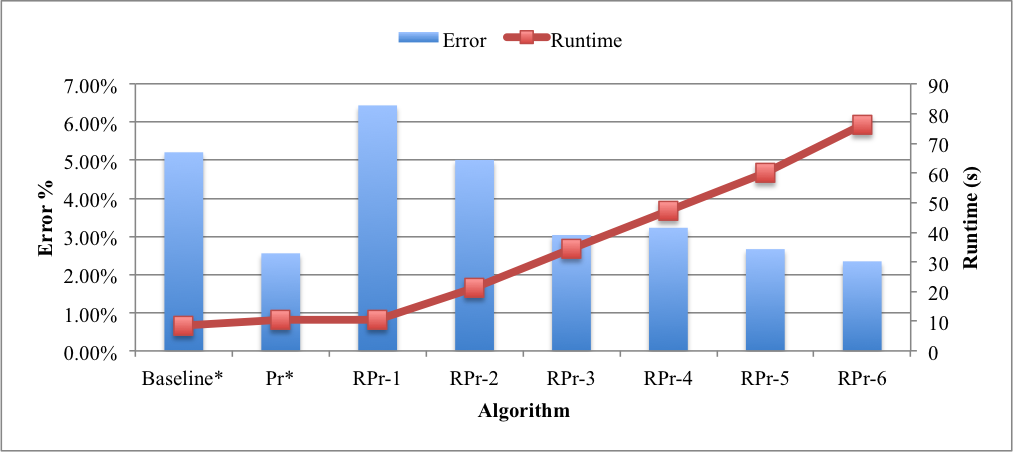
\includegraphics[scale=0.5]{fig4.png}
\caption{}
\label{exp:ms-academic-ranking}
\end{figure}


\subsection{Large-scale experiments}
Streaming correlation clustering. Show that at scale this technique can work and in a distributed environment.
In order to quantify the robustness of our methodology, we intend to run the algorithm on both synthetic and realworld datasets.
The synthetic dataset give us the ability to control the parameters while explore the state of possible responses.
However, a pitfall with such analysis is it's rather difficult to measure actual improvement over random fluctuations as well as the improvement may not be uniform across all tasks.
With experimentation on the real world datasets, we indent to first show the applicability of our method; and secondly determine whether results from our previous analysis extends to non-synthetic scenarios.


